% Generated by code/scripts/report_figures.py at 2026-10-30T09:20:59Z; do not edit.
% Inputs: artifacts/local/runs/pipeline-e2e-20261030T092022Z/run
\begin{figure}[t]
\centering
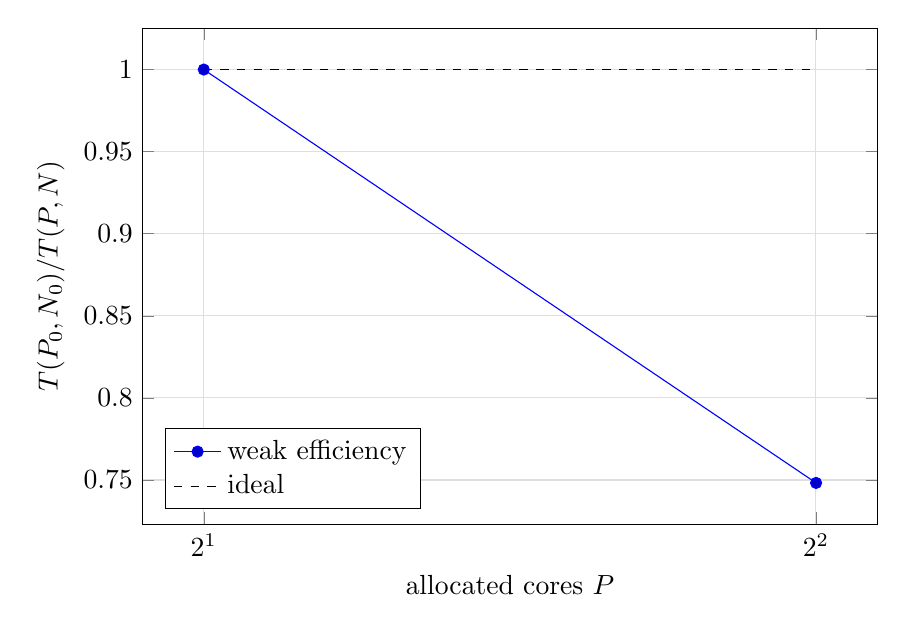
\begin{tikzpicture}
\begin{axis}[width=0.9\columnwidth, height=0.65\columnwidth, xlabel={allocated cores $P$}, ylabel={$T(P_0,N_0)/T(P,N)$}, xmode=log, log basis x=2, legend pos=south west, legend cell align=left, grid=major, grid style={gray!25}]
\addplot+[mark=*] coordinates {(2,1) (4,0.7482)};
\addlegendentry{weak efficiency}
\addplot[black, dashed] coordinates {(2,1) (4,1)};
\addlegendentry{ideal}
\end{axis}
\end{tikzpicture}
\caption{\textbf{LOCAL PIPELINE TEST, NOT A MEASUREMENT.} Weak-scaling efficiency with baseline $P_0=2$, $N_0=2000$ (1000 particles per core), threads per rank [2]. Constant particles per core is not constant work per core.}
\label{fig:weak}
\end{figure}
